\documentclass{beamer}

\usetheme{CambridgeUS}
\usecolortheme{beaver}

\setlength{\parskip}{\baselineskip}

\title{Fault Tolerance in Block-Level Caching}
\author{
  Jesus Ramos \and
  Douglas Otstott
}
\institute[FIU]{Florida International University}
\date{}

\begin{document}

\maketitle

\section{Problem Description}

\subsection{Problem Statement}

\begin{frame}
  \frametitle{Problem Statement}

  Fault tolerance in cloud systems is an important issue. Most systems
  rather than attempt to prevent failure instead expect failure and
  attempt to integrate recovery as seamlessly as possible into the system.

  Systems need to be both dependable and reliable and able to handle
  failure quickly and effectively.

  In cloud systems that employ caching, fault tolerance is a major
  issue. Currently in the event of a power or system failure all data
  that was pending to be flushed back to central storage is lost along
  with the currently cached data.

\end{frame}

% end subsection Problem Statement

\subsection{Background}

\begin{frame}
  \frametitle{Problem Background}
  
  Due to physical limitations on local storage, many large scale cloud
  based systems employ network based storage. In this scheme each host
  machine in the cloud is connected to a small number of machines
  which are responsible for the central storage in the system. This is
  known as a Storage Area Network or SAN.

  Although this solves the storage problem it introduces latency and
  bandwidth problems due to the sheer volume of requests being sent to
  the storage devices.

\end{frame}

\begin{frame}
  \frametitle{Problem Background}

  To solve this new issue of storage bandwidth and latency, most
  systems employ local caching of the most recently used data to
  reduce the number of requests that must go to central storage.

  \begin{center}
    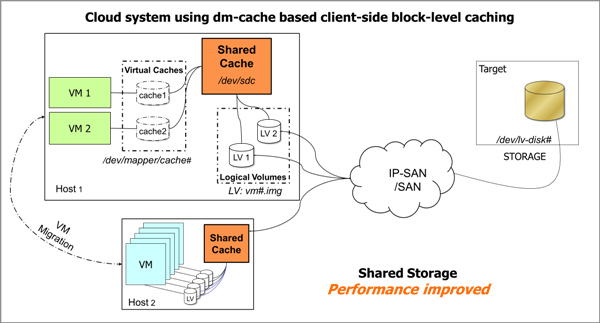
\includegraphics[scale=0.75]{../Images/NewerImage.png}
  \end{center}

\end{frame}

\begin{frame}
  \frametitle{DM-Cache}

  DM-Cache is an open source block level caching solution that was
  developed as a Linux kernel module. DM-Cache allows host machines to
  store the most recently used blocks in a designated storage device
  to reduce the number of requests to central storage systems.

  Testing so far has shown that DM-Cache alleviates network storage
  pressure in systems where numerous hosts and virtual machines create
  a bottleneck in network storage bandwidth.

  Although network storage pressure is alleviated by DM-Cache, locally
  modified blocks and current cache data is lost in the event of a
  power or system failure which can result in data loss.

\end{frame}

% end subsection Background

% end section Problem Description

\section{Proposed Solution}

\subsection{Metadata Persistence}

\begin{frame}
  \frametitle{Persist the Metadata}

  Our solution is to move the non-persistent metadata held in memory
  to the persistent cache device. This allows us to reconstruct the
  cache in the event of a system failure or power loss.

  The metadata itself will be cached in memory and written back to
  disk either when updated or at specific intervals. The trade offs of
  these methods will be evaluated for performance and fault tolerance
  of the cache.

\end{frame}

% end subsection Metadata Persistence

% end section Proposed Solution

\section{Questions}

\begin{frame}
  \frametitle{Questions?}
\end{frame}

% end section Questions

\end{document}